\documentclass[11pt]{beamer}
\usetheme{Szeged}
\usepackage[utf8]{inputenc}
\usepackage[magyar]{babel}
\usepackage[T1]{fontenc}
\usepackage{graphicx}
\usepackage{xcolor}
\graphicspath{ {./kepek/} }
\author{Tipográfiai rendszerek - \TeX}
\title{01. Bevezető}

\date{2021.02.17.} 
\subject{Órai segédanyag} 
\begin{document}

\begin{frame}
\titlepage
\end{frame}

%\begin{frame}
%\tableofcontents
%\end{frame}

\begin{frame}{Mi az a tipográfia?}
\begin{itemize}
\item A tipográfia nyomtatott betűkkel foglalkozó szakma és művészeti ág
\item Modernebb megfogalmazásban az információ megjelenítésének, valamilyen síkban megjelenített, szabályrendszere
\item A nyugati tipográfia története Gutenbergig és a nyomtatásban használható mozgatható betűk feltalálásáig nyúlik vissza
\item de az írásképek kialakítása már évezredekkel ezelőtt külön művészeti és tudományos feladatot adott az embereknek.
\end{itemize}
\end{frame}

\begin{frame}{Mi az a \TeX?}
\begin{itemize}
\item A \TeX \ (ejtsd: teh) vagy egyszerű formában TeX egy betűszedő rendszer, amelyet Donald E. Knuth készített.
\item A név a görög technê-ből ered, ezért az X (ami valójában egy nagybetűs "khi") kiejtése a "technika" „ch”-jához hasonló.
\item A \TeX \ parancsok visszafele perjellel (\textbackslash) kezdődnek és kapcsos zárójelek (\{\}) között vannak csoportosítva.
\item A \TeX \ rendszer precízen ismeri a betűk és szimbólumok méretét és ennek felhasználásával kiszámítja a lapok, a laponkénti sorok és a soronkénti karakterek optimális számát.
\item Kimenete eszközfüggetlen
	\begin{itemize}
	\item DVI
	\item PDF
	\item PS
	\end{itemize}
\end{itemize}
\end{frame}

\begin{frame}{\LaTeX}
\begin{itemize}
\item A \LaTeX \ egy \TeX-en alapuló szövegformázó rendszer, amely nagyon alkalmas olyan elektronikus dokumentumok, szakdolgozatok, tudományos cikkek írására, amelyek sok képletet tartalmaznak. 
\item A \LaTeX \ alkotója Leslie Lamport.
\end{itemize}
\end{frame}

\begin{frame}{Miért? - Előnyök}
\begin{itemize}
\item A \textit{szabad forráskód} miatt \textbf{bármilyen operációs rendszeren} használható.
\item A kész dokumentum minden szerkesztő és minden szoftveres környezet esetén azonos.
\item Nem kell foglalkozni a dokumentum megjelenésével, azt a program automatikusan szabályozza, sokkal finomabban, mint ahogy azt kézzel megtehetjük.
\end{itemize}
\end{frame}

\begin{frame}{Office csomagok}
\begin{itemize}
\item What you see is what you get
\item Amit látsz, azt kapod
\item A formázás függ a szerkesztőtől
\item más rendszeren / más szerkesztővel széteshet
\item a formázások nem koherensek - utólagos szerkesztéstől széteshet
\item Példa: sorkizárások nem megfelelő kezelése (szóközök távolsága)
\end{itemize}
\end{frame}

\begin{frame}
\begin{center}
{\Huge \textbf{TELEPÍTÉS}}
\end{center}
\end{frame}

\begin{frame}
\begin{itemize}
\item Két dolgot kell telepíteni:
	\begin{itemize}
	\item A programkörnyzetet
	\item Az editort
	\end{itemize}
\item Programkörnyezetek:
	\begin{itemize}
	\item Windows alatt: MikTeX
	\end{itemize}
\item editorok:
	\begin{itemize}
	\item TeXMaker
	\item TeXstudio
	\end{itemize}
\end{itemize}

\begin{itemize}
\item Linux alatt a telepítés egyszerűbb:
	\begin{itemize}
	\item apt install texmaker (Debian alap)
	\item dnf install texmaker (Red Hat alap)
	\item zypper install texmaker (SUSE alap)
	\item \textit{csomagkezelő} install texmaker (egyéb)
		\begin{itemize}
		\item és feltelepít mindent - környezet, függőségek, ...
		\end{itemize}
	\end{itemize}
\end{itemize}
\end{frame}

\begin{frame}
\begin{center}
{\Huge \textbf{ELSŐ LÉPÉSEK}}
\end{center}
\end{frame}

\begin{frame}{Speciális karakterek}
\begin{itemize}
\item \textbackslash \ - parancsok kezdete
\item \{ \} \ - parancsok argumentumai
\item $\left[ \right]$ - parancsok opcionális argumentumai
\item \$ - matematikai mód - képletek írásához
\item \% \ - komment - a sorban utána írt karaktereket figyelmen kívül hagyja
\item \^ \ - cirkumflex (circum flexus - fordított görbület) - hatványjel
\item \_ \ - aláhúzásjel - alsó index
\end{itemize}
\end{frame}

\begin{frame}{A forrásállomány szerkezete}
\begin{itemize}
\item \textbf{Preambulum:}
	\begin{itemize}
	\item \textbf{A forrásállomány tulajdonságai:}
	\item \textbackslash documentclass - a dokumentum típusa
	\item \textbackslash usepackage - a használt csomagok
	\item author, title, date - a dokumentum egyéb adatai
	\end{itemize}
\item \textbf{A forrásállomány törzse:}
	\begin{itemize}
	\item \textbackslash begin\{document\}-el kezdődik
	\item \textbackslash end\{document\}-el végződik
	\item amit ide írunk, az jelenik meg a fordított dokumentumban
		\begin{itemize}
		\item amit elé írunk az a preambulum részét képezi
		\item amit utána írunk az nem lesz figyelembe véve
		\end{itemize}
	\end{itemize}
\end{itemize}
\end{frame}

\begin{frame}
\begin{center}
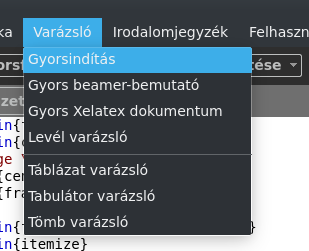
\includegraphics[scale=0.5]{k01}
\end{center}
\end{frame}

\begin{frame}
\begin{center}
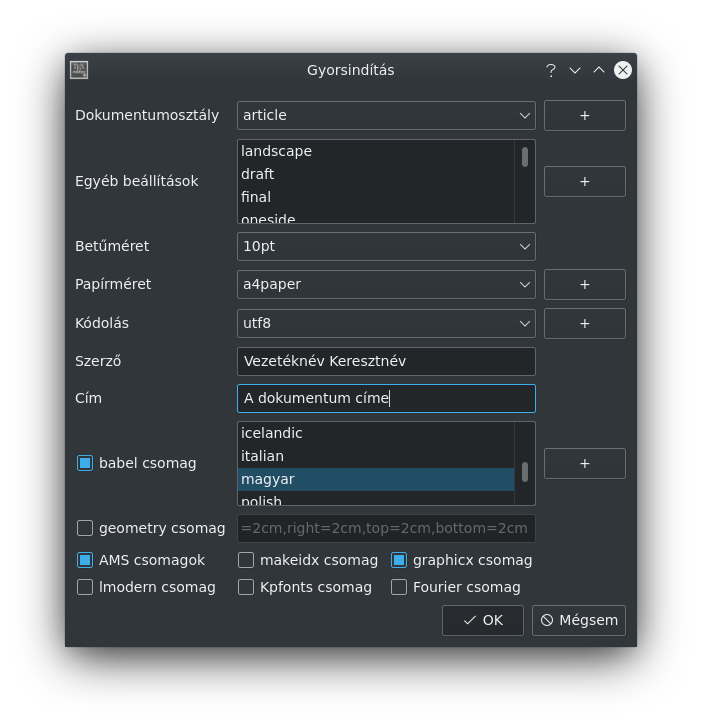
\includegraphics[scale=0.45]{k02}
\end{center}
\end{frame}

\begin{frame}
\begin{center}
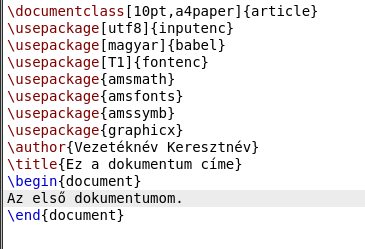
\includegraphics[scale=0.5]{k03}
\end{center}
\end{frame}

\begin{frame}{Fontosabb csomagok az induláshoz}
\begin{itemize}
\item \textbf{inputenc} - Átkódolja a forrásállományt a paraméterként kijelölt kódtáblának megfelelően.
\item \textbf{fontenc} - A \TeX \ betűkódolásának beállítása.
\item \textbf{babel} - a nyelvért / nyelvi sajátosságokért felel.
	\begin{itemize}
	\item pl. fejezetek sorszáma
	\item feladatok sorszáma a \textbf{bal} oldalon
	\end{itemize}
\end{itemize}
\end{frame}

\begin{frame}{A \TeX \ állományai}
\begin{itemize}
\item .tex - a forrásfájl
\item .log - a fordítási napló - hibakereséshez
\item .aux - címkék, idéztek, ... nyomkövetése, fordításhoz kell
\item .synctex.gz - a szerkesztőt és a pdf megjelenítőt szinkronizálja
\end{itemize}
\end{frame}

\begin{frame}{Parancsok és környezetek}
\begin{itemize}
\item	A parancsok a {\color{red}\textbackslash} -el kezdődnek
\item	A környezetek a {\color{blue}\textbackslash begin\{név\}}-el kezdődnek
\item	és a {\color{blue}\textbackslash end\{név\}} -el végződnek
\end{itemize}
\end{frame}

\begin{frame}{Hibák és figyelmeztetések}
\begin{itemize}
\item {\color{red}Hibák} - kritikusak - nem fordul a forrás (logikai)
\item {\color{blue}Figyelmeztetések} - fordul a forrás, csak valami nem oké (szemantikai)
\end{itemize}
\end{frame}

\begin{frame}{Források:}
\begin{itemize}
\item Wikipédia: \TeX \ és \LaTeX
\item T. OETIKER, H. PARTL, I. HYNA, E. SCHLEGL: Egy nem túl rövid bevezető a \LaTeX \ 2$\varepsilon$ használatába
\end{itemize}
\end{frame}

\end{document}